% Created by tikzDevice version 0.12 on 2019-03-21 22:03:49
% !TEX encoding = UTF-8 Unicode
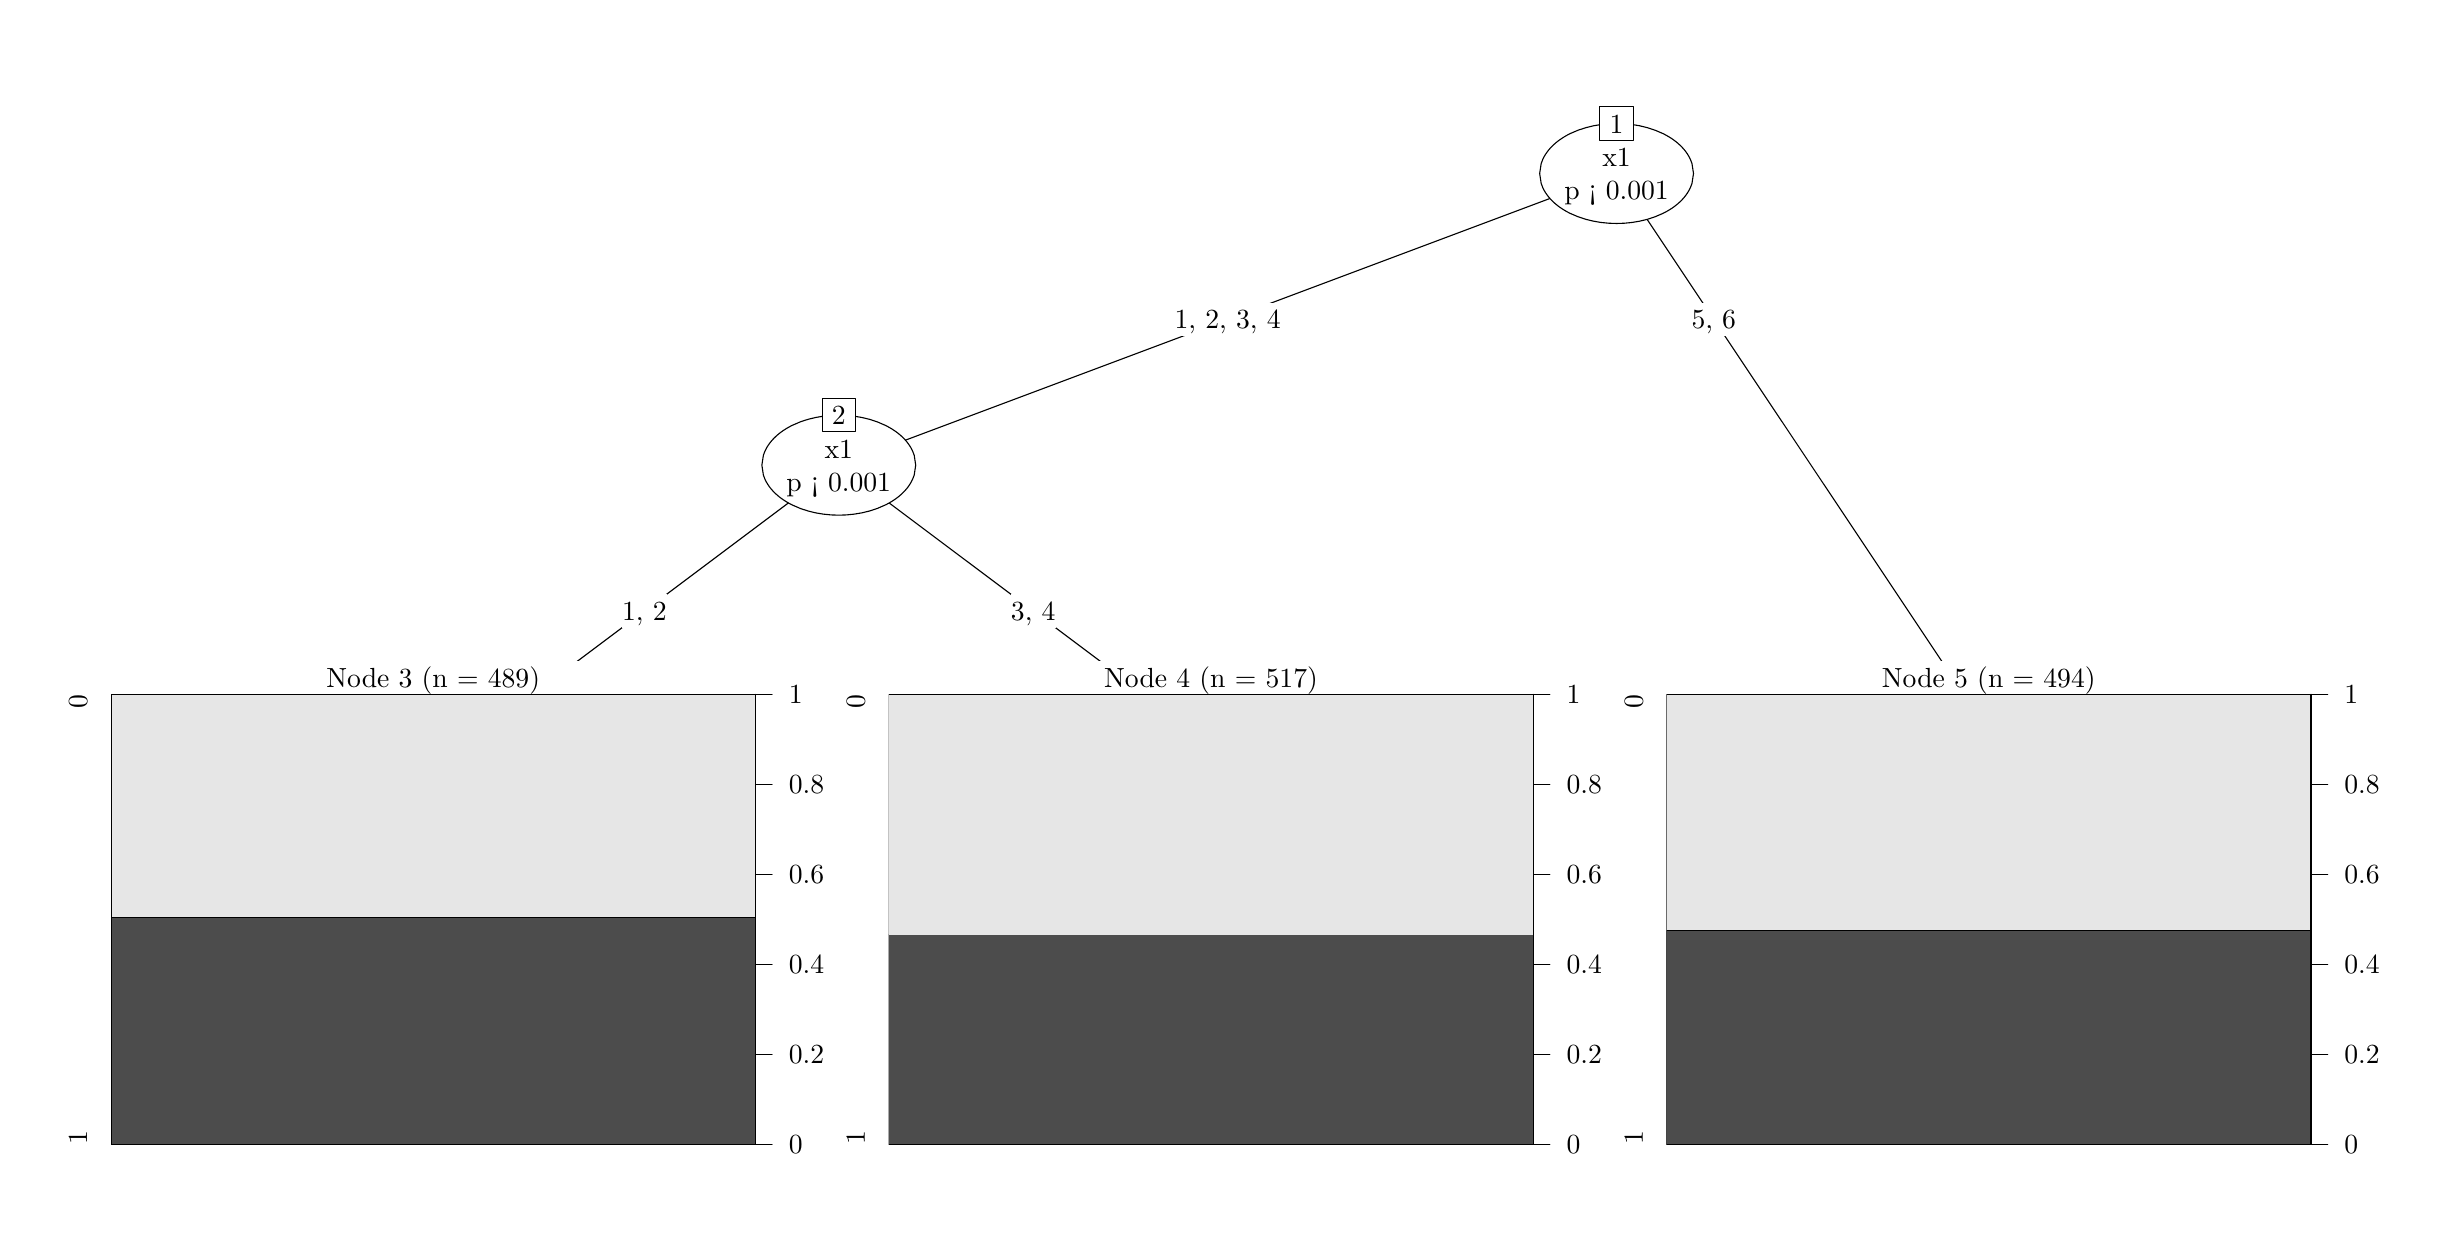
\begin{tikzpicture}[x=1pt,y=1pt]
\definecolor{fillColor}{RGB}{255,255,255}
\path[use as bounding box,fill=fillColor,fill opacity=0.00] (0,0) rectangle (867.24,433.62);
\begin{scope}
\path[clip] (  0.00,  0.00) rectangle (867.24,433.62);
\definecolor{drawColor}{RGB}{0,0,0}

\path[draw=drawColor,line width= 0.4pt,line join=round,line cap=round] (574.14,380.92) --
	(293.09,275.53);

\path[draw=drawColor,line width= 0.4pt,line join=round,line cap=round] (574.14,380.92) --
	(714.67,170.14);
\definecolor{fillColor}{RGB}{255,255,255}

\path[draw=drawColor,line width= 0.4pt,line join=round,line cap=round,fill=fillColor] (546.35,380.92) --
	(546.90,384.52) --
	(547.46,385.98) --
	(548.01,387.09) --
	(548.57,388.00) --
	(549.13,388.80) --
	(549.68,389.50) --
	(550.24,390.14) --
	(550.79,390.73) --
	(551.35,391.26) --
	(551.91,391.76) --
	(552.46,392.23) --
	(553.02,392.67) --
	(553.57,393.08) --
	(554.13,393.46) --
	(554.69,393.83) --
	(555.24,394.17) --
	(555.80,394.50) --
	(556.35,394.81) --
	(556.91,395.10) --
	(557.47,395.38) --
	(557.47,395.38) --
	(560.25,396.57) --
	(563.03,397.48) --
	(565.81,398.16) --
	(568.59,398.63) --
	(571.37,398.90) --
	(574.14,398.99) --
	(576.92,398.90) --
	(579.70,398.63) --
	(582.48,398.16) --
	(585.26,397.48) --
	(588.04,396.57) --
	(590.82,395.38) --
	(590.82,395.38) --
	(591.38,395.10) --
	(591.94,394.81) --
	(592.49,394.50) --
	(593.05,394.17) --
	(593.60,393.83) --
	(594.16,393.46) --
	(594.72,393.08) --
	(595.27,392.67) --
	(595.83,392.23) --
	(596.38,391.76) --
	(596.94,391.26) --
	(597.50,390.73) --
	(598.05,390.14) --
	(598.61,389.50) --
	(599.16,388.80) --
	(599.72,388.00) --
	(600.28,387.09) --
	(600.83,385.98) --
	(601.39,384.52) --
	(601.94,380.92) --
	(601.94,380.92) --
	(601.39,377.33) --
	(600.83,375.86) --
	(600.28,374.76) --
	(599.72,373.84) --
	(599.16,373.05) --
	(598.61,372.34) --
	(598.05,371.70) --
	(597.50,371.12) --
	(596.94,370.58) --
	(596.38,370.08) --
	(595.83,369.62) --
	(595.27,369.18) --
	(594.72,368.77) --
	(594.16,368.38) --
	(593.60,368.02) --
	(593.05,367.68) --
	(592.49,367.35) --
	(591.94,367.04) --
	(591.38,366.75) --
	(590.82,366.47) --
	(590.82,366.47) --
	(588.04,365.28) --
	(585.26,364.36) --
	(582.48,363.69) --
	(579.70,363.22) --
	(576.92,362.95) --
	(574.14,362.86) --
	(571.37,362.95) --
	(568.59,363.22) --
	(565.81,363.69) --
	(563.03,364.36) --
	(560.25,365.28) --
	(557.47,366.47) --
	(557.47,366.47) --
	(556.91,366.75) --
	(556.35,367.04) --
	(555.80,367.35) --
	(555.24,367.68) --
	(554.69,368.02) --
	(554.13,368.38) --
	(553.57,368.77) --
	(553.02,369.18) --
	(552.46,369.62) --
	(551.91,370.08) --
	(551.35,370.58) --
	(550.79,371.12) --
	(550.24,371.70) --
	(549.68,372.34) --
	(549.13,373.05) --
	(548.57,373.84) --
	(548.01,374.76) --
	(547.46,375.86) --
	(546.90,377.33) --
	(546.35,380.92) --
	cycle;

\node[text=drawColor,anchor=base,inner sep=0pt, outer sep=0pt, scale=  1.00] at (574.14,383.50) {x1};

\node[text=drawColor,anchor=base,inner sep=0pt, outer sep=0pt, scale=  1.00] at (574.14,371.46) {p < 0.001};

\path[draw=drawColor,line width= 0.4pt,line join=round,line cap=round,fill=fillColor] (568.12,392.97) rectangle (580.17,405.01);

\node[text=drawColor,anchor=base,inner sep=0pt, outer sep=0pt, scale=  1.00] at (574.14,395.55) {1};
\end{scope}
\begin{scope}
\path[clip] (  0.00,  0.00) rectangle (867.24,433.62);
\definecolor{fillColor}{RGB}{255,255,255}

\path[fill=fillColor] (414.46,322.20) rectangle (452.78,334.25);
\definecolor{drawColor}{RGB}{0,0,0}

\node[text=drawColor,anchor=base,inner sep=0pt, outer sep=0pt, scale=  1.00] at (433.62,324.78) {1, 2, 3, 4};
\end{scope}
\begin{scope}
\path[clip] (  0.00,  0.00) rectangle (867.24,433.62);
\definecolor{fillColor}{RGB}{255,255,255}

\path[fill=fillColor] (601.22,322.20) rectangle (617.33,334.25);
\definecolor{drawColor}{RGB}{0,0,0}

\node[text=drawColor,anchor=base,inner sep=0pt, outer sep=0pt, scale=  1.00] at (609.28,324.78) {5, 6};
\end{scope}
\begin{scope}
\path[clip] (  0.00,  0.00) rectangle (867.24,433.62);
\definecolor{drawColor}{RGB}{0,0,0}

\path[draw=drawColor,line width= 0.4pt,line join=round,line cap=round] (293.09,275.53) --
	(152.57,170.14);

\path[draw=drawColor,line width= 0.4pt,line join=round,line cap=round] (293.09,275.53) --
	(433.62,170.14);
\definecolor{fillColor}{RGB}{255,255,255}

\path[draw=drawColor,line width= 0.4pt,line join=round,line cap=round,fill=fillColor] (265.30,275.53) --
	(265.85,279.12) --
	(266.41,280.59) --
	(266.96,281.69) --
	(267.52,282.61) --
	(268.08,283.40) --
	(268.63,284.11) --
	(269.19,284.75) --
	(269.74,285.33) --
	(270.30,285.87) --
	(270.86,286.37) --
	(271.41,286.84) --
	(271.97,287.27) --
	(272.52,287.68) --
	(273.08,288.07) --
	(273.64,288.43) --
	(274.19,288.78) --
	(274.75,289.10) --
	(275.30,289.41) --
	(275.86,289.71) --
	(276.42,289.98) --
	(276.42,289.98) --
	(279.20,291.18) --
	(281.98,292.09) --
	(284.76,292.76) --
	(287.54,293.23) --
	(290.32,293.51) --
	(293.09,293.60) --
	(295.87,293.51) --
	(298.65,293.23) --
	(301.43,292.76) --
	(304.21,292.09) --
	(306.99,291.18) --
	(309.77,289.98) --
	(309.77,289.98) --
	(310.33,289.71) --
	(310.89,289.41) --
	(311.44,289.10) --
	(312.00,288.78) --
	(312.55,288.43) --
	(313.11,288.07) --
	(313.67,287.68) --
	(314.22,287.27) --
	(314.78,286.84) --
	(315.33,286.37) --
	(315.89,285.87) --
	(316.45,285.33) --
	(317.00,284.75) --
	(317.56,284.11) --
	(318.11,283.40) --
	(318.67,282.61) --
	(319.23,281.69) --
	(319.78,280.59) --
	(320.34,279.12) --
	(320.89,275.53) --
	(320.89,275.53) --
	(320.34,271.93) --
	(319.78,270.47) --
	(319.23,269.37) --
	(318.67,268.45) --
	(318.11,267.65) --
	(317.56,266.95) --
	(317.00,266.31) --
	(316.45,265.73) --
	(315.89,265.19) --
	(315.33,264.69) --
	(314.78,264.22) --
	(314.22,263.79) --
	(313.67,263.38) --
	(313.11,262.99) --
	(312.55,262.63) --
	(312.00,262.28) --
	(311.44,261.96) --
	(310.89,261.65) --
	(310.33,261.35) --
	(309.77,261.08) --
	(309.77,261.08) --
	(306.99,259.88) --
	(304.21,258.97) --
	(301.43,258.29) --
	(298.65,257.83) --
	(295.87,257.55) --
	(293.09,257.46) --
	(290.32,257.55) --
	(287.54,257.83) --
	(284.76,258.29) --
	(281.98,258.97) --
	(279.20,259.88) --
	(276.42,261.08) --
	(276.42,261.08) --
	(275.86,261.35) --
	(275.30,261.65) --
	(274.75,261.96) --
	(274.19,262.28) --
	(273.64,262.63) --
	(273.08,262.99) --
	(272.52,263.38) --
	(271.97,263.79) --
	(271.41,264.22) --
	(270.86,264.69) --
	(270.30,265.19) --
	(269.74,265.73) --
	(269.19,266.31) --
	(268.63,266.95) --
	(268.08,267.65) --
	(267.52,268.45) --
	(266.96,269.37) --
	(266.41,270.47) --
	(265.85,271.93) --
	(265.30,275.53) --
	cycle;

\node[text=drawColor,anchor=base,inner sep=0pt, outer sep=0pt, scale=  1.00] at (293.09,278.11) {x1};

\node[text=drawColor,anchor=base,inner sep=0pt, outer sep=0pt, scale=  1.00] at (293.09,266.06) {p < 0.001};

\path[draw=drawColor,line width= 0.4pt,line join=round,line cap=round,fill=fillColor] (287.07,287.57) rectangle (299.12,299.62);

\node[text=drawColor,anchor=base,inner sep=0pt, outer sep=0pt, scale=  1.00] at (293.09,290.15) {2};
\end{scope}
\begin{scope}
\path[clip] (  0.00,  0.00) rectangle (867.24,433.62);
\definecolor{fillColor}{RGB}{255,255,255}

\path[fill=fillColor] (214.78,216.81) rectangle (230.89,228.85);
\definecolor{drawColor}{RGB}{0,0,0}

\node[text=drawColor,anchor=base,inner sep=0pt, outer sep=0pt, scale=  1.00] at (222.83,219.39) {1, 2};
\end{scope}
\begin{scope}
\path[clip] (  0.00,  0.00) rectangle (867.24,433.62);
\definecolor{fillColor}{RGB}{255,255,255}

\path[fill=fillColor] (355.30,216.81) rectangle (371.41,228.85);
\definecolor{drawColor}{RGB}{0,0,0}

\node[text=drawColor,anchor=base,inner sep=0pt, outer sep=0pt, scale=  1.00] at (363.36,219.39) {3, 4};
\end{scope}
\begin{scope}
\path[clip] (  0.00,  0.00) rectangle (867.24,433.62);
\definecolor{fillColor}{RGB}{255,255,255}

\path[fill=fillColor] ( 12.05, 30.11) rectangle (293.10,204.76);
\definecolor{drawColor}{RGB}{0,0,0}

\node[text=drawColor,anchor=base,inner sep=0pt, outer sep=0pt, scale=  1.00] at (146.55,195.30) {Node 3 (n = 489)};
\end{scope}
\begin{scope}
\path[clip] (  0.00,  0.00) rectangle (867.24,433.62);
\definecolor{drawColor}{RGB}{0,0,0}

\node[text=drawColor,rotate= 90.00,anchor=base west,inner sep=0pt, outer sep=0pt, scale=  1.00] at ( 21.51, 30.11) {1};

\node[text=drawColor,rotate= 90.00,anchor=base east,inner sep=0pt, outer sep=0pt, scale=  1.00] at ( 21.51,192.72) {0};

\path[draw=drawColor,line width= 0.4pt,line join=round,line cap=round] (262.98, 30.11) --
	(262.98,192.72);

\path[draw=drawColor,line width= 0.4pt,line join=round,line cap=round] (262.98, 30.11) -- (269.00, 30.11);

\path[draw=drawColor,line width= 0.4pt,line join=round,line cap=round] (262.98, 62.63) -- (269.00, 62.63);

\path[draw=drawColor,line width= 0.4pt,line join=round,line cap=round] (262.98, 95.16) -- (269.00, 95.16);

\path[draw=drawColor,line width= 0.4pt,line join=round,line cap=round] (262.98,127.68) -- (269.00,127.68);

\path[draw=drawColor,line width= 0.4pt,line join=round,line cap=round] (262.98,160.20) -- (269.00,160.20);

\path[draw=drawColor,line width= 0.4pt,line join=round,line cap=round] (262.98,192.72) -- (269.00,192.72);

\node[text=drawColor,anchor=base west,inner sep=0pt, outer sep=0pt, scale=  1.00] at (275.03, 26.67) {0};

\node[text=drawColor,anchor=base west,inner sep=0pt, outer sep=0pt, scale=  1.00] at (275.03, 59.19) {0.2};

\node[text=drawColor,anchor=base west,inner sep=0pt, outer sep=0pt, scale=  1.00] at (275.03, 91.71) {0.4};

\node[text=drawColor,anchor=base west,inner sep=0pt, outer sep=0pt, scale=  1.00] at (275.03,124.23) {0.6};

\node[text=drawColor,anchor=base west,inner sep=0pt, outer sep=0pt, scale=  1.00] at (275.03,156.75) {0.8};

\node[text=drawColor,anchor=base west,inner sep=0pt, outer sep=0pt, scale=  1.00] at (275.03,189.28) {1};
\end{scope}
\begin{scope}
\path[clip] ( 30.11, 30.11) rectangle (262.98,192.72);
\definecolor{drawColor}{RGB}{0,0,0}

\path[draw=drawColor,line width= 0.4pt,line join=round,line cap=round] ( 30.11, 30.11) rectangle (262.98,192.72);
\definecolor{fillColor}{gray}{0.30}

\path[draw=drawColor,line width= 0.4pt,line join=round,line cap=round,fill=fillColor] ( 30.11, 30.11) rectangle (262.98,112.25);
\definecolor{fillColor}{RGB}{230,230,230}

\path[fill=fillColor] ( 30.11,112.25) rectangle (262.98,192.72);

\path[draw=drawColor,line width= 0.4pt,line join=round,line cap=round] ( 30.11, 30.11) rectangle (262.98,192.72);
\end{scope}
\begin{scope}
\path[clip] (  0.00,  0.00) rectangle (867.24,433.62);
\definecolor{fillColor}{RGB}{255,255,255}

\path[fill=fillColor] (293.10, 30.11) rectangle (574.14,204.76);
\definecolor{drawColor}{RGB}{0,0,0}

\node[text=drawColor,anchor=base,inner sep=0pt, outer sep=0pt, scale=  1.00] at (427.60,195.30) {Node 4 (n = 517)};
\end{scope}
\begin{scope}
\path[clip] (  0.00,  0.00) rectangle (867.24,433.62);
\definecolor{drawColor}{RGB}{0,0,0}

\node[text=drawColor,rotate= 90.00,anchor=base west,inner sep=0pt, outer sep=0pt, scale=  1.00] at (302.56, 30.11) {1};

\node[text=drawColor,rotate= 90.00,anchor=base east,inner sep=0pt, outer sep=0pt, scale=  1.00] at (302.56,192.72) {0};

\path[draw=drawColor,line width= 0.4pt,line join=round,line cap=round] (544.03, 30.11) --
	(544.03,192.72);

\path[draw=drawColor,line width= 0.4pt,line join=round,line cap=round] (544.03, 30.11) -- (550.06, 30.11);

\path[draw=drawColor,line width= 0.4pt,line join=round,line cap=round] (544.03, 62.63) -- (550.06, 62.63);

\path[draw=drawColor,line width= 0.4pt,line join=round,line cap=round] (544.03, 95.16) -- (550.06, 95.16);

\path[draw=drawColor,line width= 0.4pt,line join=round,line cap=round] (544.03,127.68) -- (550.06,127.68);

\path[draw=drawColor,line width= 0.4pt,line join=round,line cap=round] (544.03,160.20) -- (550.06,160.20);

\path[draw=drawColor,line width= 0.4pt,line join=round,line cap=round] (544.03,192.72) -- (550.06,192.72);

\node[text=drawColor,anchor=base west,inner sep=0pt, outer sep=0pt, scale=  1.00] at (556.08, 26.67) {0};

\node[text=drawColor,anchor=base west,inner sep=0pt, outer sep=0pt, scale=  1.00] at (556.08, 59.19) {0.2};

\node[text=drawColor,anchor=base west,inner sep=0pt, outer sep=0pt, scale=  1.00] at (556.08, 91.71) {0.4};

\node[text=drawColor,anchor=base west,inner sep=0pt, outer sep=0pt, scale=  1.00] at (556.08,124.23) {0.6};

\node[text=drawColor,anchor=base west,inner sep=0pt, outer sep=0pt, scale=  1.00] at (556.08,156.75) {0.8};

\node[text=drawColor,anchor=base west,inner sep=0pt, outer sep=0pt, scale=  1.00] at (556.08,189.28) {1};
\end{scope}
\begin{scope}
\path[clip] (311.16, 30.11) rectangle (544.03,192.72);
\definecolor{drawColor}{RGB}{0,0,0}

\path[draw=drawColor,line width= 0.4pt,line join=round,line cap=round] (311.16, 30.11) rectangle (544.03,192.72);
\definecolor{fillColor}{gray}{0.30}

\path[draw=drawColor,line width= 0.4pt,line join=round,line cap=round,fill=fillColor] (311.16, 30.11) rectangle (544.03,105.91);
\definecolor{fillColor}{RGB}{230,230,230}

\path[fill=fillColor] (311.16,105.91) rectangle (544.03,192.72);

\path[draw=drawColor,line width= 0.4pt,line join=round,line cap=round] (311.16, 30.11) rectangle (544.03,192.72);
\end{scope}
\begin{scope}
\path[clip] (  0.00,  0.00) rectangle (867.24,433.62);
\definecolor{fillColor}{RGB}{255,255,255}

\path[fill=fillColor] (574.14, 30.11) rectangle (855.19,204.76);
\definecolor{drawColor}{RGB}{0,0,0}

\node[text=drawColor,anchor=base,inner sep=0pt, outer sep=0pt, scale=  1.00] at (708.65,195.30) {Node 5 (n = 494)};
\end{scope}
\begin{scope}
\path[clip] (  0.00,  0.00) rectangle (867.24,433.62);
\definecolor{drawColor}{RGB}{0,0,0}

\node[text=drawColor,rotate= 90.00,anchor=base west,inner sep=0pt, outer sep=0pt, scale=  1.00] at (583.61, 30.11) {1};

\node[text=drawColor,rotate= 90.00,anchor=base east,inner sep=0pt, outer sep=0pt, scale=  1.00] at (583.61,192.72) {0};

\path[draw=drawColor,line width= 0.4pt,line join=round,line cap=round] (825.08, 30.11) --
	(825.08,192.72);

\path[draw=drawColor,line width= 0.4pt,line join=round,line cap=round] (825.08, 30.11) -- (831.11, 30.11);

\path[draw=drawColor,line width= 0.4pt,line join=round,line cap=round] (825.08, 62.63) -- (831.11, 62.63);

\path[draw=drawColor,line width= 0.4pt,line join=round,line cap=round] (825.08, 95.16) -- (831.11, 95.16);

\path[draw=drawColor,line width= 0.4pt,line join=round,line cap=round] (825.08,127.68) -- (831.11,127.68);

\path[draw=drawColor,line width= 0.4pt,line join=round,line cap=round] (825.08,160.20) -- (831.11,160.20);

\path[draw=drawColor,line width= 0.4pt,line join=round,line cap=round] (825.08,192.72) -- (831.11,192.72);

\node[text=drawColor,anchor=base west,inner sep=0pt, outer sep=0pt, scale=  1.00] at (837.13, 26.67) {0};

\node[text=drawColor,anchor=base west,inner sep=0pt, outer sep=0pt, scale=  1.00] at (837.13, 59.19) {0.2};

\node[text=drawColor,anchor=base west,inner sep=0pt, outer sep=0pt, scale=  1.00] at (837.13, 91.71) {0.4};

\node[text=drawColor,anchor=base west,inner sep=0pt, outer sep=0pt, scale=  1.00] at (837.13,124.23) {0.6};

\node[text=drawColor,anchor=base west,inner sep=0pt, outer sep=0pt, scale=  1.00] at (837.13,156.75) {0.8};

\node[text=drawColor,anchor=base west,inner sep=0pt, outer sep=0pt, scale=  1.00] at (837.13,189.28) {1};
\end{scope}
\begin{scope}
\path[clip] (592.21, 30.11) rectangle (825.08,192.72);
\definecolor{drawColor}{RGB}{0,0,0}

\path[draw=drawColor,line width= 0.4pt,line join=round,line cap=round] (592.21, 30.11) rectangle (825.08,192.72);
\definecolor{fillColor}{gray}{0.30}

\path[draw=drawColor,line width= 0.4pt,line join=round,line cap=round,fill=fillColor] (592.21, 30.11) rectangle (825.08,107.47);
\definecolor{fillColor}{RGB}{230,230,230}

\path[fill=fillColor] (592.21,107.47) rectangle (825.08,192.72);

\path[draw=drawColor,line width= 0.4pt,line join=round,line cap=round] (592.21, 30.11) rectangle (825.08,192.72);
\end{scope}
\end{tikzpicture}
